% -*- TeX-PDF-mode: t -*-

% Template for ICASSP-2010 paper; to be used with:
%          spconf.sty  - ICASSP/ICIP LaTeX style file, and
%          IEEEbib.bst - IEEE bibliography style file.
% --------------------------------------------------------------------------
\documentclass{article}
\usepackage{spconf,amsmath,graphicx}
\usepackage{url}
\usepackage{verbatim}
\usepackage{subfig}
%\usepackage{microtype}

% Example definitions.
% --------------------
\def\x{{\mathbf x}}
\def\L{{\cal L}}

\usepackage{color}
\newcommand{\FIXME}[2][FIXME]{\textcolor{blue}{\textbf{#1}: \emph{#2}}}

% Title.
% ------
%\title{IMPUTATION OF BEAT-ALIGNED FEATURES AND MUSIC PATTERN LEARNING}
\title{EVALUATING MUSIC SEQUENCE MODELS THROUGH MISSING DATA}
%
% Single address.
% ---------------
%\name{Thierry Bertin-Mahieux\thanks{Thanks to NSERC and some other stuff.}}
%\address{EE dept., Columbia University}
%
% For example:
% ------------
%\address{School\\
%	Department\\
%	Address}
%
% Two addresses (uncomment and modify for two-address case).
% ----------------------------------------------------------
\twoauthors {Thierry Bertin-Mahieux\sthanks{supported in part by a
    NSERC PG scholarship.}, Graham Grindlay} {Columbia University\\
  LabROSA\\ New York, USA} {Ron J. Weiss\sthanks{supported by NSF
    grant IIS-0844654 and Institute of Museum and Library Services
    grant LG-06-08-0073-08.} and Daniel P.W. Ellis} {New York
  University / Columbia University\\ MARL / LabROSA\\ New York, USA}

\begin{document}
\ninept
%
\maketitle
%
\begin{abstract}
  We investigate the task of missing data imputation in music signals
  as a means of evaluating the ability of different signal models to
  accurately capture the temporal structure present in music.
  %
  We analyze beat-synchronous chromagrams and compare linear ??? ...
  %
  Simple predictive models perform best when measured using a
  Euclidean distance metric, despite producing results which are not
  musically meaningful.  We therefore investigate alternate evaluation
  measures which emphasize musical consistency....
%

Gives a reasonable benchmark to compare algorithms that claim learning meaningful
temporal patterns on music. Hard to beat benchmarks comparison, for instance linear
prediction. We compare some methods and discuss contradicting error measures. 
\end{abstract}
%
\begin{keywords}
Missing data, chroma features, beat imputation, codebook learning
\end{keywords}
%

% NSF thanks
\makeatletter{\renewcommand*{\@makefnmark}{}
\footnotetext{This work is supported by NSF grant
    IIS-0713334 and by a gift from Google, Inc.
    Any opinions, findings and conclusions or
    recommendations expressed in this material are those of the
    authors and do not necessarily reflect the views of the sponsors.}\makeatother}

\section{Introduction}
\label{sec:intro}
As with many classes of time-series data, musical signals contain
substantial amounts of complex structural information.  Given the
intricate nature of this data, learning models of music in an
unsupervised fashion is a particularly challenging task.  In addition
to musicological implications, large-scale models of music data have
numerous commercial applications, including recommendation systems,
digital rights management, and creative tools.  For many applications
we are interested in models that capture local patterns
(i.e. ``patches'') in the data.  Finding robust sequential patterns
may prove useful for tasks such as song similarity (recognizing songs
with similar patterns), song segmentation (labeling chorus/verse
structure), and cover song recognition (identifying songs with similar
high-level patterns).  All of these tasks would benefit from patch
models that exhibit high-level musical characteristics while remaining
faithful to the observed signal data.
%\FIXME[gg]{Do we need to back this up more?}
%Therefore, we are interested in patterns that not only explain the
%low-level signal, but also contain musical characteristics.  
However, it is unclear how to evaluate the quality of this type of
model.  In this paper, we propose a task based on missing data
imputation and discuss various performance metrics which are sensitive
to musically meaningful aspects of the data.

Imputation refers to a family of techniques used to fill in missing
data entries.  Previous work on audio-related applications has
included speech denoising~\cite{Raj1998}, source
separation~\cite{Reyes-Gomez2005}, bandwidth
expansion~\cite{Smaragdis2009}, and model
evaluation~\cite{Hoffman2010}.  However, much of the
previous work has focused on at most a single time-frame.
%However, to the best of
%our knowledge, previous research has only considered at most a single
%missing time frame.
%a few missing time-frequency \emph{bins}
%\FIXME[ronw]{this isn't totally fair, some of the missing
%  data speech stuff is based on imputation using HMM/CRF models. E.g. see
%  figure 3 of
%  {\footnotesize \url{http://www.ee.columbia.edu/~mjr59/AISTATS-defspec.pdf}}
%}.
The single-frame imputation problem is often somewhat easy since the
harmonic content of music tends to change more slowly than a single
frame.  However as the length of missing data increases, the problem
becomes significantly more challenging.
%
We therefore focus on the task of \emph{multi-frame} imputation in
% many consecutive time frames
which long segments of the signal are missing.
%
Obtaining good performance on this task requires the use of a model
which takes advantage of the highly structured nature of music.  It
therefore serves as a good way to
% This allows us to
more carefully evaluate the temporal aspects of competing
models.  % needs to be reworded?
% mention real-world packet-loss case?


% Music is highly structured in time and as such is particularly suitable
% for the multi-frame imputation task.
% In addition to musicological implications,
% large-scale models of music data have numerous commercial
% applications, including recommendation systems, digital rights
% management, and creative tools.  



\begin{comment}
and fully masking consecutive beats of music have not been
considered. A real-life analogous problem would be a music stream
signal that is lost for a few seconds. The goal here would be to infer
a reasonable stream to replace the original one. Thus we do not only
want a signal close to the original in a reconstruction sense, but
also a signal that has similar ``musical properties'' to the user
ear. These properties are difficult to define, but we refer to higher
order dependencies present in the signal. For instance, the rate of
note onsets, the number of notes activated at the same time, and other
texture-like elements. We will argue that entropy is a good
approximation of these characteristics.
\end{comment}

\begin{comment}
a few frequency bins are hidden and can be
recovered from their neighborhood, both in time and frequency. Masking
one full beat is a natural extension, and the solution is easy as
music notes are often sustained over many beats. Two or three missing
beats remain solvable as music bare many repetitions. One can usually
find a similar section from an unmasked part of the song (think about
a repeated chorus for instance).  The real challenge arises from
masking many consecutive beats.
\end{comment}


The difficult nature of multi-frame imputation of music data is
demonstrated in Figure \ref{fig:basic}.
%
Linear regression\FIXME[ronw]{or prediction?}, which explicitly
minimizes Euclidean distance, is used to impute the missing data in
Figure~\ref{fig:basic}.  However, it is clear from visual inspection
that linear regression yields an overly-smooth reconstruction and is
unable to predict the temporal evolution within the missing section.
%
A more sophisticated signal model which better leverages the
surrounding context and makes use of long-term temporal information
such as knowledge of repetitions within a song (note that the
missing sequence is repeated at frame 70) is necessary to achieve a musically
coherent reconstruction.
%
Unfortunately, simple algorithms such as linear regression
are often prone to identifying poor solutions, despite optimizing standard
metrics such as Euclidean distance.
%
In this paper, we argue that a more extensive set of metrics is needed
to properly evaluate a model's ability to predict musical sequences.
%more for proper evaluation.


\section{TASK DEFINITION}
\label{sec:task}

\subsection{DATA AND FEATURES}
\label{ssec:feats}
In the experiments described below, we use a set of $5000$ songs taken
from the \emph{morecowbell.dj} dataset~\cite{Bertin-Mahieux2010a}.
This dataset contains a wide variety of (predominantly western) pop
music.  The raw audio was then converted to a chromagram
representation using the online EchoNest
API.\footnote{\url{http://developer.echonest.com}} A chromagram is
similar in spirit to a constant-Q spectrogram except that pitch
content across all octaves has been folded into $12$ discrete bins,
each of which corresponds to a semitone (e.g. piano key).
%In the chroma representation, the pitch content at each point in time
%is folded into a $12$ binsintensity associated with each of the 12
%semitones (e.g. piano keys) across all octaves.
%
%One can see them as a very coarse %and noisy
%and low dimensional music transcription which captures the harmonic
%content of the signal while ignoring information related to timbre and
%instrumentation.  
%We use an online API\footnote{\url{http://developer.echonest.com}} %
%\cite{EchoNest} 
%that computes chroma from a constant-Q spectrogram.

Music naturally evolves over a time scale expressed in beats, as
opposed to the fixed-length frames commonly used in other audio
processing applications.  Beat-aligned chroma can be formed by
resampling a chromagram so that each chroma (column) vector spans a
single beat.  This representation has been successfully used for cover
song recognition~\cite{Ellis2007a}, segmentation~\cite{Weiss2010}, and
in our previous work on patch modeling~\cite{Bertin-Mahieux2010a}.  As
a post-processing step, we remove variability due to loudness by
normalizing each column to have a maximum value of $1$.

% ronw: this sentence is unnecessary
% Note
%that music beat tracking algorithms perform relatively well
%\cite{Davies2007} even if the task is not considered solved.

%Beat-aligned chroma features have been used for cover song recognition
%\cite{Ellis2007a} and segmentation \cite{Weiss2010}. In our previous work
%\cite{Bertin-Mahieux2010a}, we attempt to learn music patterns in that
%representation.
% Results on multi-frame imputation are done on
%In the following sections we report experimental results over 
%a random
%subset of $5000$ songs from the morecowbell.dj dataset
%\cite{Bertin-Mahieux2010a}.


%\begin{figure}[t]
%\begin{center}
%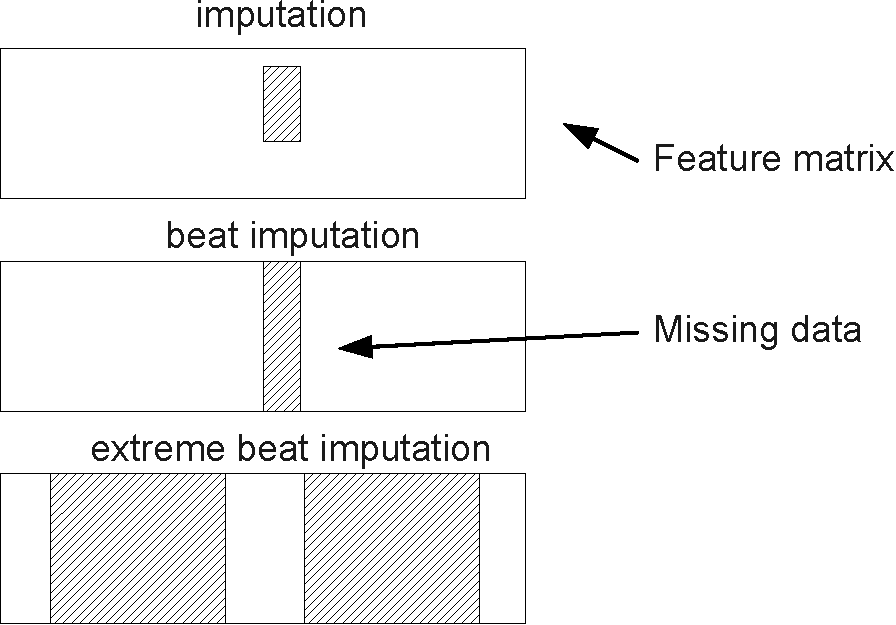
\includegraphics[width=.7\columnwidth]{type_imputation}
%\end{center}
%\caption{Imputation types.
%\label{fig:types}}
%\end{figure}

\begin{figure}[t]
\begin{center}
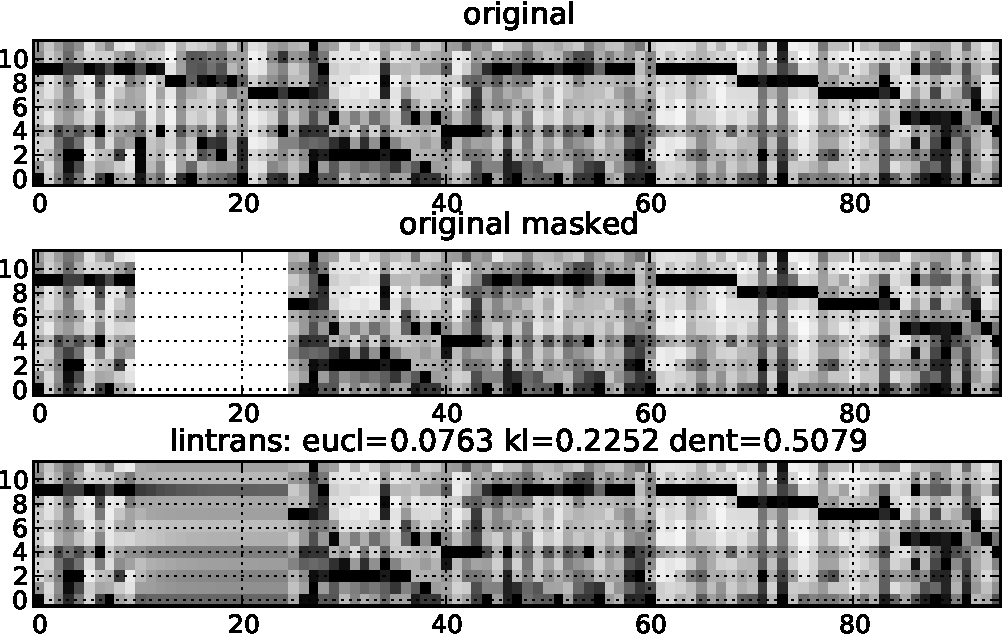
\includegraphics[width=.95\columnwidth]{basic}
\end{center}
\caption{$15$ beats imputation example, rows are 1) original 2) original masked
3) reconstruction using a linear transform of one previous beat.
\label{fig:basic}}
\end{figure}

% IPYTHON COMMAND TO RECREATE ABOVE FIGURE
%btchroma2 = sio.loadmat('/home/thierry/Columbia/covers80/coversongs/covers32kENmats/john_lennon+Double_Fantasy+05-I_m_Losing_You.mp3.mat')['btchroma']
%p1=185;p2=p1+15;mask=np.ones(btchroma2.shape);mask[:,p1:p2]=0.
%evaluation.plot_oneexample(btchroma2,mask,p1,p2,methods=['lintrans'],methods_args=[{'win':1}],measures=('eucl','kl','dent'),plotrange=(p1-10,p2+70))


%\subsection{MEASURES}
\subsection{EVALUATION METRICS}
\label{ssec:measures}
Euclidean distance is a natural first choice for reconstruction and
encoding tasks. However, as can be seen in Figure \ref{fig:basic},
algorithms which minimize this metric do not necessarily capture all
of the relevant data statistics.  In particular, the solution is
overly smooth and longer-term temporal patterns are poorly
reconstructed.

Clearly, the simplicity of the model is largely responsible for these
issues.  However, inherent in the Euclidean distance criterion is a
preference for smooth solutions.
%There is no doubt that this poor reconstruction is in part due to
%the simplicity of the model. That said, we argue that minimizing
%Euclidean distance also leads to such reconstructions, i.e. when 
%a model is unsure of a value, it gets the most reward from a smooth
%solution.
To see why, consider the toy example of Figure \ref{fig:square}. We
impute the original one-dimensional signal, a square wave (solid
line), by two signals: a translated identical square wave (dot-dashed
line), and a constant signal (dashed line). The first signal has an
average reconstruction error of $0.50$ using Euclidean distance. The
second signal has an average error of only $0.25$, despite the fact
that it does not appear to reflect the overall shape of the original
data.

%Applied to a multidimensional signal, it implies that Euclidean
%distance rewards overly-smoothed reconstruction, thus it can be
%misleading.

The class of Minkowski distances are given by the form $d_p =
|x_1-x_2|^p$, of which the Euclidean is a special case ($p=2$).  In
general, as $p \rightarrow 0$ the resulting distance measures penalize
small values more heavily.  This has the effect of favoring
``sharper'' data sequences and is illustrated in Figure
\ref{fig:measures}.  The greyed rectangle represents the case where a
reconstruction is considered valid if it is between some $\delta$ of
the original and wrong otherwise.  The Minkowski distance approximates
this case with an increasingly smaller $\delta$ as $p \rightarrow 0$.
In the experiments described below, we consider $p=0.5$ and $p=2$.
%\FIXME[ronw]{elaborate on this, it's kind of unclear}

Looking at the differences between the original data and the imputed
values, it appears that we need to encourage sparsity in our
solutions.  Entropy is a natural measure of the sparsity of a
distribution and therefore it makes sense to consider related metrics.
We examined the (symmetric) Kullback-Leibler divergence, (approximate)
conditional entropy~\cite{}, Jensen difference~\cite{Michel1994}, and
the normalize difference entropy (\textbf{D-ENT})
\cite{Mentzelopoulos2004}.

Another idea is to look at the histogram of values and compute its
entropy.  Once again, sustained solutions should measure differently
than the original.  Absolute normalize difference entropy
(\textbf{D-ENT}) \cite{Mentzelopoulos2004} between two vectors is
computed as follow: we discretize $(0,1)$ in $10$ bins and create the
normalized histogram of values.  The entropy of each of the bins
$b_{bi}$ is $e_b = - log_2 b_b$ for each of the two vectors
$i$. Finally:
\[
\mbox{D-ENT} = \left( \Sigma_b \frac{e_{b1} - e_{b2}}{e_{b1}} \right) / (\mbox{\# bins})
\]
Note that D-ENT is not symmetric. In our experiment, the first vector
is the original one.  If we look at Figure \ref{fig:avgnnrand}, the
reconstruction with the lowest D-ENT is using nearest neighbor and not
averaging as with Euclidean distance.

Note that we tried other entropy related measures,
i.e. Kullback-Leibler divergence (KL) and Jensen difference
\cite{Michel1994}. As for $d_{1/2}$, they behave in a surprisingly
similar fashion as the Euclidean distance.  We explained above why
Euclidean distance justifies disappointing reconstructions. At the
same time, we do not argue that we should ignore or replace
it. Euclidean distance measures reconstruction in a fundamental
way. We believe we need a set of measures to quantify the quality of
music patterns, Euclidean distance being one of them. In the next
section, we investigate which measures behave in a similar way, thus
helping us to decide which ones are useful to report.

\begin{comment}
The smoothing phenomena described above explains why reconstruction
such as in Figure \ref{fig:basic} ($3$rd row) or in Figure
\ref{fig:avgnnrand} ($3$rd row) may occur.  Learning an overly
smoothed solution and avoiding extreme values is rewarded by some
metrics.  Figure~\ref{fig:square} suggests that $d_{1/2}$ might
perform well for real imputation tasks

$d_{1/2}$ seems to be a solution from the toy example in
Figure \ref{fig:square}, but we will see in Section \ref{sec:exp} that
it is not really the case in practice.  Similarly, Kullback-Leibler
(KL), conditional entropy and Jensen difference \cite{Michel1994} are
two measures based on entropy, thus should not behave necessarily in
the same way as $d_p$.  Once again, it is not the case in practice. We
now look into other measures that would differ from $d_2$.  Upon
visual inspection, they should reward granularity which is missing in
Figure \ref{fig:basic} for instance. Delta chromas are the finite
difference along the time axis of the chromas. Deltas of over-smoothed
solution are closed to $0$ whereas features of typical songs have more
variation over time.  \textbf{ddiff} measures the absolute difference
between the sum of absolute values of the deltas for the original data
and its reconstruction.
\end{comment}

\begin{figure}[t]
\begin{center}
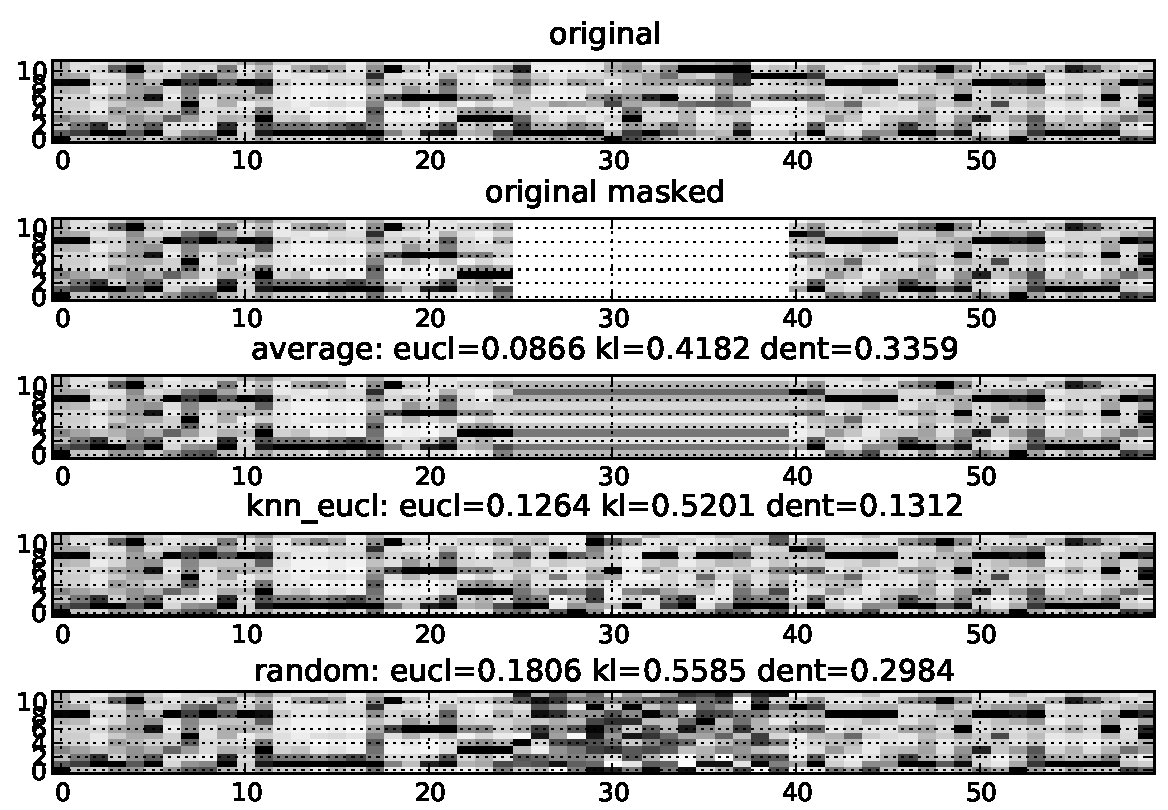
\includegraphics[width=.95\columnwidth]{avg_nn_rand}
\end{center}
\caption{Same beat imputation example as Figure \ref{fig:basic}, 
rows are 1) original 2) original masked
3) reconstruction using the average of nearby beats 4) using
nearest neighbor 5) using random.
\label{fig:avgnnrand}}
\end{figure}


\begin{figure}%
\centering
\subfloat[]{%
\label{fig:measures}%
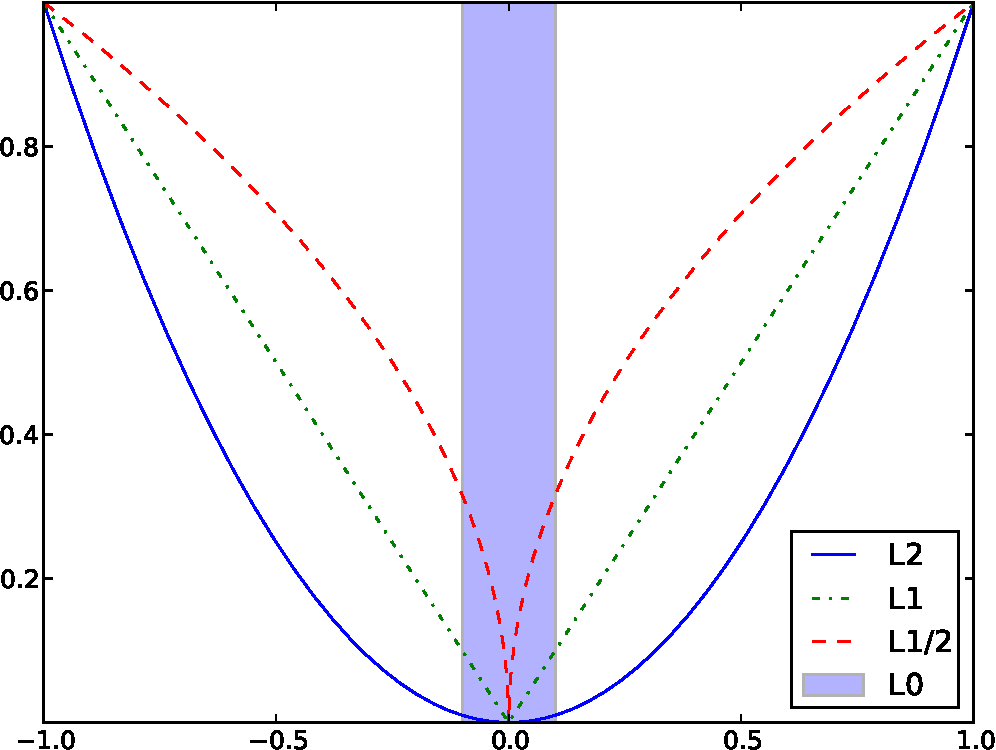
\includegraphics[width=0.485\columnwidth]{measures}} 
\hspace{0.1cm}
\subfloat[]{%
\label{fig:square}%
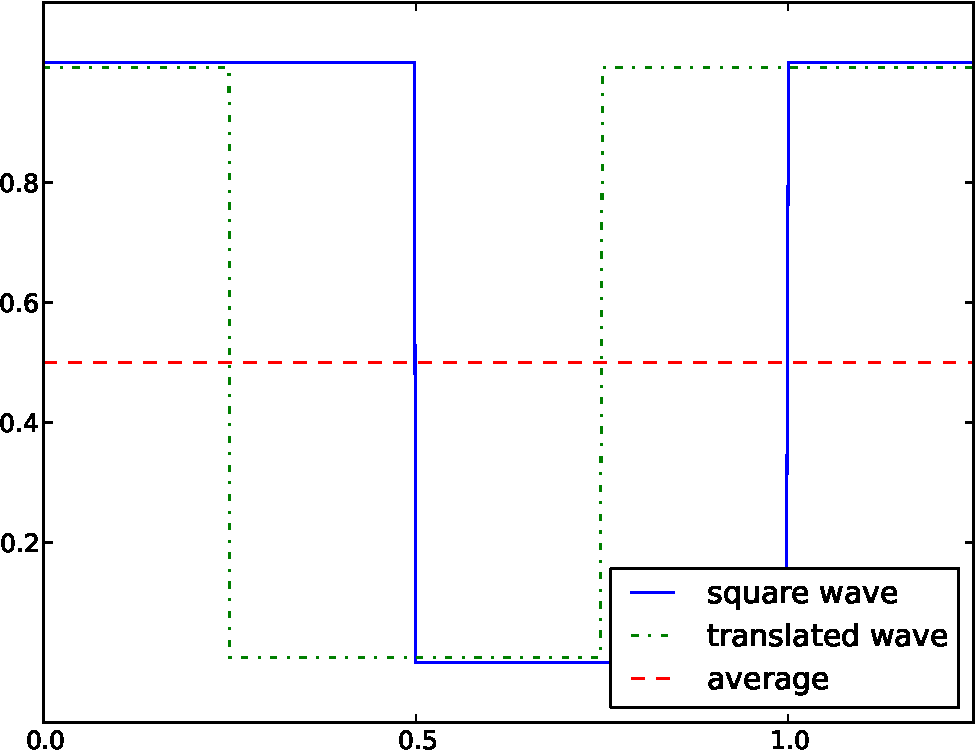
\includegraphics[width=0.475\columnwidth]{square}}%
\hspace{8pt}%
\caption{(a) Effect of different measures on one-dimensional data. (b)
  Reconstruction error between a square wave and two approximations, a
  square wave translated by a quarter of the period, and the average
  function. Average error between original and translated wave is
  always $0.5$ for any Minkowski measure $d_p$ on $[0,1]$.  For the
  average function, the errors are $0.25$, $0.5$ and $0.71$ for $d_2$,
  $d_1$ and $d_{1/2}$ respectively.}%
\label{fig:two_measures}
\end{figure}


\begin{comment}
  Reconstruction error between a square wave and two approximations, a
  square wave translated by a quarter of the period, and the average
  function. Average error between original and translated wave is
  always $0.5$ for any Minkowski measure $d_p$ on $[0,1]$.  For the
  average function, the errors are $0.25$, $0.5$ and $0.71$ for $d_2$,
  $d_1$ and $d_{1/2}$ respectively.
\end{comment}


\section{EXPERIMENTS}
\label{sec:exp}
We present results from different algorithms for imputing masked
beats.  Features are beat-aligned chromas and the dataset is made of
$5000$ songs from the morecowbell.dj dataset
\cite{Bertin-Mahieux2010a}. Songs has to be of length at least $100$
beats.  The masked part is chosen at random, excluding the first and
last $30$ beats.


\subsection{ALGORITHMS}
\label{ssec:algo}
As multi-frame imputation has not been studied before, we report
results on a variety of benchmark algorithms. We realize that such
methods have a low probability of success at solving the task, but
their relative performance is of interest.  Simple methods include
\textbf{random} where each chroma bin is drawn from a uniform $[0,1)$
distribution (Figure \ref{fig:avgnnrand}, $5$th row).  One can also
pick a beat at random from the song, or take the average of all
visible beats. Taking the \textbf{average} of the beats within a certain
range of the missing patch (Figure \ref{fig:avgnnrand}, $3$rd row)
create a smooth reconstruction, but still solves the case of
sustained notes.

Our first trained model is linear regression (called \textbf{linear
  transform} in
the text) where we use $N$ previous beats to predict the next one.  As
it explicitly learns to minimize Euclidean distance on the visible
data, this methods performs very well under certain metrics (See
Figure \ref{fig:basic}). From our experiments, $N=1$ or $N=2$ work
best.

Nearest neighbor ($\mathbf{1}$\textbf{NN}) is an appropriate tehcnique
to take advantage of the repetitions within a song. By looking at the
nearby beats of the missing data, we can impute a reconstruction by
spotting a similar neighborhood. Note that instead of using the
visible part of the song, one can use a \textbf{codebook} made of
other songs.  $k$NN with $k>1$ is ongoing research.

Previous methods rely on local, low-level information which should not
be enough to solve multi-frame imputation. HMM or NMF should better
leverage long term dependencies and nearby information.  We experiment
with shift invariant probabilistic latent component analysis
(\textbf{SIPLCA}) \cite{Smaragdis2009,Weiss2010}, a probabilistic
version of NMF. SIPLCA learn how to encode the signal as overlapping
patches. The missing data is inferred by maximizing expectation.
Problems arise when the number of missing beats is larger than the
patch size. SIPLCA can activate patches or not without any
penalty. Thus, we regularize the the activation by applying a second
level of SIPLCA.  Still, results are not impressive and improvements
are part of our ongoing research. We refer the interested reader to
our code for more details.



\subsection{RESULTS}
\label{ssec:results}
As we mentioned in Subsection \ref{ssec:measures}, many metrics reward
reconstructions in a very similar fashion. The Euclidean distance is
often the default choice for many tasks, and we will see that many
others measures tend to agree with it. At the same time, measures like
delta difference and D-ENT offer another perspective. We try to
rationalize this idea by measuring the correlation between our
metrics. Pearson's correlation is defined as
\[  \rho_{X,Y}=\mathrm{corr}(X,Y)={\mathrm{cov}(X,Y) \over \sigma_X
    \sigma_Y} ={E[(X-\mu_X)(Y-\mu_Y)] \over \sigma_X\sigma_Y}
\]
$\rho_{X,Y}$. Remember that $-1 \leq \rho_{X,Y} \leq 1$, an absolute
value close to $1$ meaning high correlation. $\rho_{X,Y}$ is computed
for many error measures based on results obtained by three methods on
two multi-frame imputation tasks. See results in Table
\ref{tab:corrs}. Delta difference and D-ENT stand out as measuring
things differently than Euclidean distance.

% MEASURES IN ORDER: (bad matfile saving)
%array(['condent', 'binary', 'cos', 'eucl', 'lhalf', 'lhalf_delta', 'dent',
%       'thresh', 'thresh_delta', 'cos_delta', 'jdiff', 'kl', 'ddiff',
%       'eucl_delta', 'leven'], 
%      dtype='|S12')
\begin{table}[t]
\begin{small}
\begin{center}
\begin{tabular}{|l|c|c|c|c|c|} \hline
 & Eucl. & $d_{1/2}$ & Jensen & Delta diff. & D-ENT \\ \hline
Eucl. & $1$ & $0.90$ & $0.84$ & $0.21$ & $0.12$ \\ 
$d_{1/2}$. & $0.90$ & $1$ & $0.71$ & $0.22$ & $0.27$ \\ 
Jensen & $0.84$ & $0.71$ & $1$ & $-0.04$ & $0.20$ \\ \hline 
Delta diff. & $\mathbf{0.21}$ & $0.22$ & $-0.04$ & $1$ & -$0.02$ \\ 
D-ENT & $\mathbf{0.12}$ & $0.27$ & $0.20$ & $-0.02$ & $1$ \\ \hline
cos & $0.88$ & $0.76$ & $0.97$ & $-0.03$ & $0.20$ \\
KL & $0.77$ & $0.64$ & $0.95$ & $-0.04$ & $0.17$ \\ 
cond. ent. & $0.58$ & $0.68$ & $0.37$ & $0.32$ & $0.18$ \\
thresh. & $0.68$ & $0.91$ & $0.51$ & $0.20$ & $0.35$ \\ \hline
\end{tabular}
\caption{Pearson correlation between measures. Based on all results
  from random, average, $1$NN and linear transform on $5000$K songs
  with $1$ and $10$ missing beats. $1$ or $-1$ means high correlation,
  $0$ means none. ``Jensen'' is Jensen difference, ``cos'' is cosine
  distance, ``cond. ent.'' is conditional entropy, ``thresh.'' is the
  greyed area measure from Figure \ref{fig:measures} with $\delta =
  0.2$.
\label{tab:corrs}}
\end{center}
\end{small}
\end{table}

We take a closer look at this divergence between measures in Figure
\ref{fig:2dscore}.  It shows the performance of three methods for
different numbers of missing beats. We report Euclidean distance and
D-ENT. Nearest neighbor (NN) method creates a reconstruction with a
granularity similar to the original for all mask sizes. We can assume
that D-ENT is approximately constant throughout a song. Thus, a
imputation from NN preserve this characteristic.  Regarding the linear
transform, it learns to minimize the Euclidean distance and does it
successfully. But as it can be seen with D-ENT and in Figure
\ref{fig:basic} $3$rd row, it is done by a large amount of
smoothing. The average reconstruction has the same granularity than
the linear transform, but due to less smoothing (or a less intelligent
one), it does not do as well with the Euclidean distance.

\begin{figure}[t]
\begin{center}
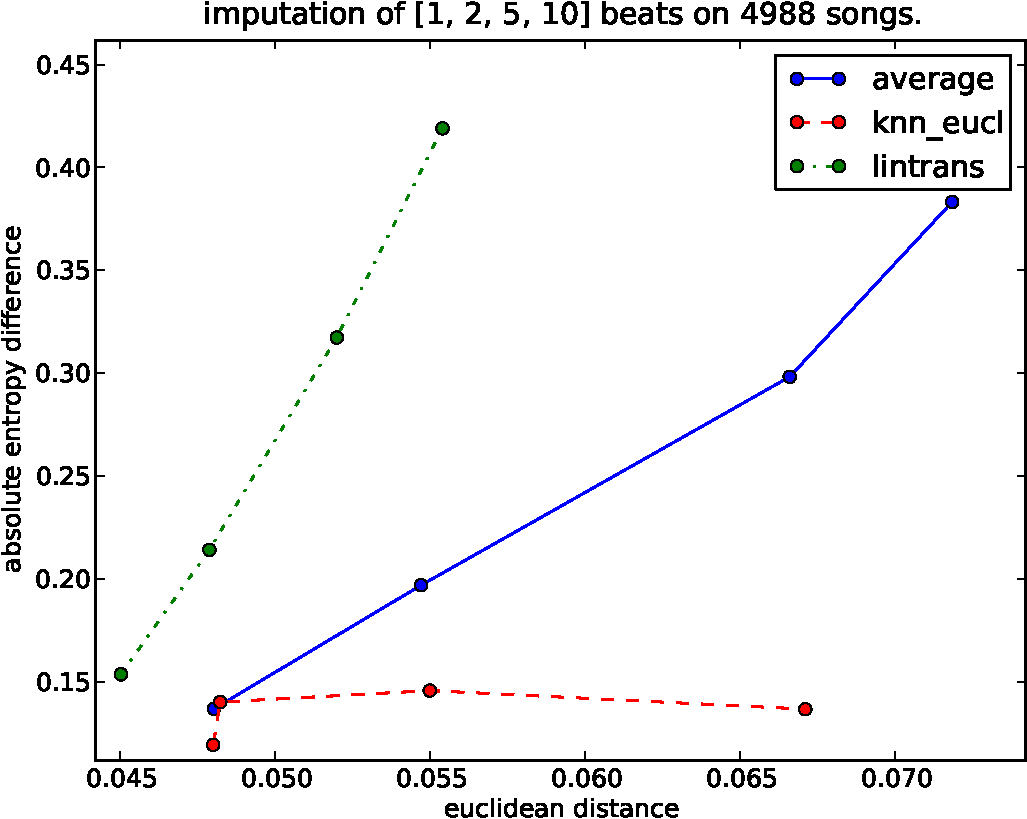
\includegraphics[width=.9\columnwidth]{recon_score_in_2d_5k}
\end{center}
\caption{Reconstruction error for $3$ methods and different
number of masked beats. Errors are D-ENT and Euclidean
distance. In all cases, the larger the number of masked beats,
the higher the Euclidean distance. Lower left is better.
\label{fig:2dscore}}
\end{figure}

We now report results of a $15$ beat imputation on $5000$ songs in
Table \ref{tab:res}. The linear transform is a clear winner based on
Euclidean distance. As before, nearest neighbor's strength is to
preserve the texture of the original patch as can be seen from his
D-ENT score. We can not present all results (other number of missing
beats, oter error measures, etc) due to space constraints, but they
are no serious surprises with other measures as can be expected from
Table \ref{tab:corrs}.

\begin{table}[t]
\begin{small}
\begin{center}
\begin{tabular}{|l||c|c|c|} \hline
method & Euclidean & delta diff. & D-ENT \\ \hline
random & $0.168$ & $$ & $0.252$ \\
average & $0.079$ & $$ & $0.430$ \\ \hline
1NN & $0.072$ & $$ & $\mathbf{0.123}$ \\
codebook & & & \\ \hline
lin. trans. & $\mathbf{0.056}$ & $$ & $0.479$ \\
SIPLCA & & & \\ \hline
\end{tabular}
\caption{Results on $15$ missing beats by different methods
on $5000$ songs and measured using Euclidean distance and
D-ENT.
\label{tab:res}}
\end{center}
\end{small}
\end{table}

In Figure \ref{fig:origrecon} we present specific examples of original
/ reconstruction pairs. Pay attention to the D-ENT values and the fact
that it prefers the second reconstruction.  It is due to a similar
repartition of graey-scale values troughout the patch. Once again,
this measure favors NN-like methods. Note also that delta difference
tends to reward overly-granular solution, as it is the only measure to
prefer the $3$rd reconstruction to the $2$nd one. Finally, the
reconstruction by SIPLCA is in our opinion an example of a
reconstruction that visually makes sense but get disppointing results.

\begin{figure}[t]
\begin{center}
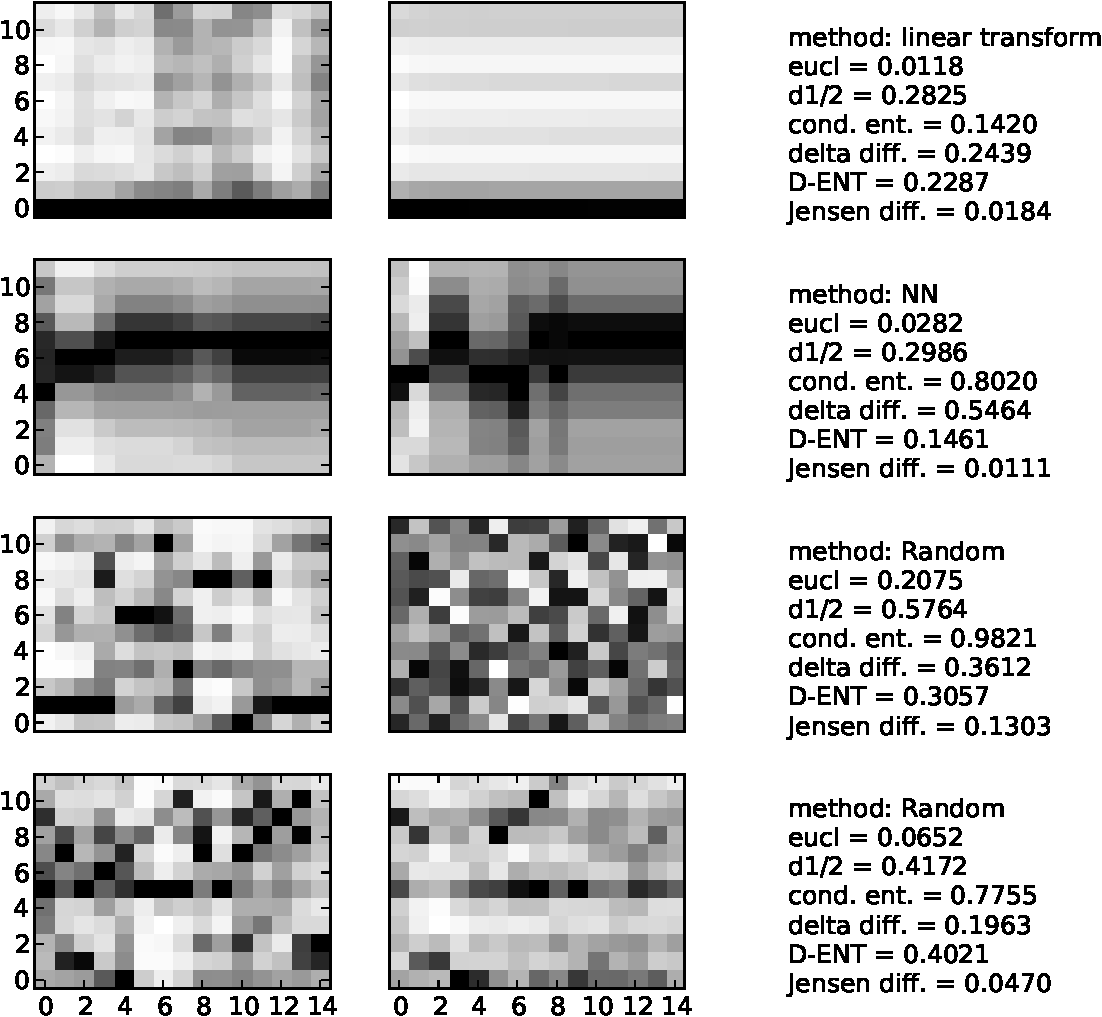
\includegraphics[width=.9\columnwidth]{original_recons}
\end{center}
\caption{Selected pairs of original patches ($1$st column)
and their reconstructions ($2$nd column). 
Method used and some error measures
reported on the right.
\label{fig:origrecon}}
\end{figure}

\section{CONCLUSION AND FUTURE WORK}
\label{sec:conclusion}
As mentioned, modifications of HMM and SIPLCA are ongoing
research. There is great hope that algorithms pretrained
on large additional data (another set of songs) will break
the curse of boring smoothed patterns.
A unified set of measures should also be selected
by the community. Our code and test data is available to 
reproduce and improve these results.

Code available at \url{http://www.columbia.edu/~tb2332/proj/imputation.html}.


%\section{ACKNOWLEDGEMENTS}
%NSERC PG grant for Thierry, something for Ron, NSF from Dan.


% References should be produced using the bibtex program from suitable
% BiBTeX files (here: strings, refs, manuals). The IEEEbib.bst bibliography
% style file from IEEE produces unsorted bibliography list.
% -------------------------------------------------------------------------
\bibliographystyle{IEEEbib}
\bibliography{tbm_bib}

\end{document}
